\subsection{Aprendizaje automático}

El aprendizaje automático es una rama de la inteligencia artificial que se centra en el desarrollo de algoritmos y modelos estadísticos que capacitan a los sistemas informáticos para mejorar su desempeño en tareas específicas mediante la experiencia adquirida a partir del procesamiento de datos \cite{elgendy2020deep}. Estos sistemas están diseñados para aprender, predecir y tomar decisiones basadas en el análisis de conjuntos extensos de datos, identificando patrones y adaptándose a nuevas situaciones sin requerir programación explícita \cite{goodfellow2016deep}.

El impacto del aprendizaje automático se extiende ampliamente en la actualidad, siendo fundamental en diversas aplicaciones como búsquedas en la web, filtrado de contenido en redes sociales y recomendaciones en plataformas de comercio electrónico \cite{geron2019hands}. Asimismo, se ha integrado en sistemas inteligentes como cámaras y dispositivos móviles, autos autónomos, vehículos aéreos no tripulados, y otros relacionados a la visión por computador \cite{patterson2017deep}.

Los algoritmos de aprendizaje automático tienen fundamentos en la estadística, en la optimización, en la teoría de la información y en la computación, y según su forma de aprender, estos pueden clasificarse en tres grupos: aprendizaje supervisado, aprendizaje no supervisado y aprendizaje por refuerzo \cite{goodfellow2016deep}.

\subsubsection{Aprendizaje supervisado}

En el aprendizaje supervisado, los algoritmos se entrenan sobre conjuntos de datos etiquetados, los cuales representan las soluciones deseadas. A estos datos se les conoce como etiquetas, lo que significa que cada ejemplo de entrenamiento está emparejado con una salida (etiqueta o valor de respuesta) \cite{geron2019hands}. El objetivo es que el algoritmo aprenda a predecir la etiqueta a partir de las características de los datos de entrada \cite{patterson2017deep}.

Tras el entrenamiento, se evalúa el algoritmo con datos no vistos durante la fase de aprendizaje para verificar su capacidad de generalización \cite{geron2019hands}. Las tareas comunes para este tipo de aprendizaje son la regresión, que busca predecir un valor numérico continuo, y la clasificación, que busca dividir los datos en subgrupos en base a sus características (ver Figura ~\ref{fig:supervised}).

\begin{figure}[H]
    \begin{center}
        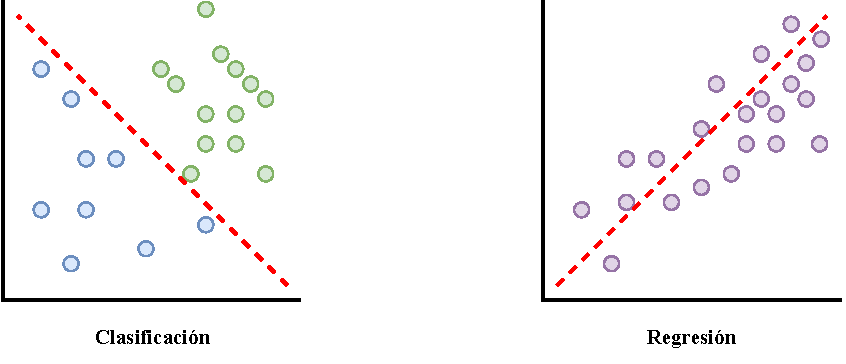
\includegraphics[width=0.9\textwidth]{Images/supervised.pdf}
    \end{center}
    \caption{Diferencias entre un problema de clasificación y un problema de regresión.}
    \reference{Elaborado por el autor.}
    \label{fig:supervised}
\end{figure}

Según \citeA{geron2019hands}, los algoritmos supervisados más importantes son: regresión lineal, regresión logística, maquina de vectores de soporte, árboles de decisión y bosques aleatorios, k vecinos cercanos y las redes neuronales.

\subsubsection{Aprendizaje no supervisado}

Los algoritmos de aprendizaje no supervisado se distinguen del aprendizaje supervisado por prescindir de conjuntos de datos etiquetados. En lugar de ello, el sistema busca comprender las estructuras y los patrones inherentes a los datos sin una orientación explícita hacia un resultado específico  \cite{geron2019hands}. Este enfoque encuentra aplicaciones en diversas tareas, como la detección de anomalías, como se observa en las máquinas de vectores de soporte de una clase; la reducción de la dimensionalidad, ejemplificada en el análisis de componentes principales; y principalmente, en el agrupamiento o clustering (ver Figura~\ref{fig:clustering}), donde se destacan métodos como K-medias, DBSCAN y análisis de conglomerados.

\begin{figure}[H]
    \begin{center}
        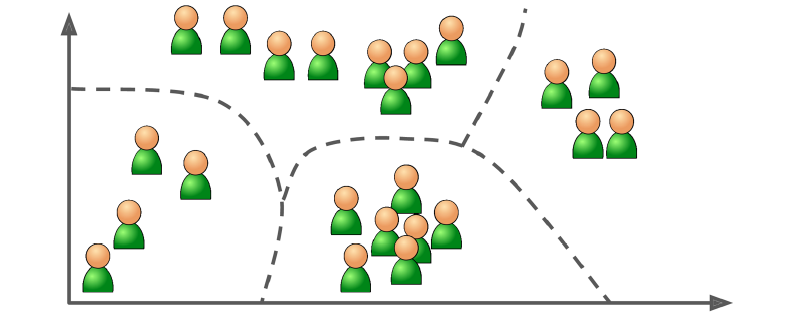
\includegraphics[width=1\textwidth]{Images/clustering.png}
    \end{center}
    \caption{Agrupamiento (clustering).}
    \reference{Datos tomados de \citeA{geron2019hands}.}
    \label{fig:clustering}
\end{figure}

\subsubsection{Aprendizaje por refuerzo}

Este tipo de aprendizaje se enfoca en la maximización de una métrica de recompensa acumulada, dictando cómo los agentes deben operar dentro de un entorno dado. A través de iteraciones de prueba y error, el agente adquiere estrategias adaptables, permitiéndole ajustar sus acciones a contextos específicos con el fin de alcanzar sus metas \cite{geron2019hands}.
